\documentclass[xcolor=dvipsnames,class=article,a4paper]{beamer}

%\documentclass[notes]{beamer}            Folien und Notizen anzeigen
% \documentclass[notes=only]{beamer}  nur Notizen anzeigen
%\documentclass{beamer}                      nur Folien anzeigen
\setbeamerfont{note page}{size=\scriptsize} % Schriftgröße der Notizseiten ändern (default: \small)

\usepackage[ngerman]{babel}
\usepackage[utf8]{inputenc}
\usepackage{color}
\usepackage[dvipsnames]{xcolor}
\usepackage{colortbl}
\usepackage{tabularx}
\usepackage{multirow}
\usepackage{array} % wird für Einstellungen bei Tabellen benötigt
\usepackage{amsmath}
\usepackage{mathtools}
\usepackage{wrapfig}
\usepackage{pdfpages}
\usepackage{booktabs} % für horizontale Linien innerhalb von aligned (in equations)

% Bearbeiten der Umgebung, mit Hilfe derer R-Codes im Text dargestellt werden
% Der Befehl zum Einbinden der Codes: \lstinputlisting{Datei.R}
\usepackage{listings}
\lstset{ 
  language=R,                     % the language of the code
  basicstyle=\scriptsize\ttfamily, % the size of the fonts that are used for the code
  numbers=none,                   % where to put the line-numbers (z.B. 'numbers=left')
  numberstyle=\footnotesize\color{Blue},  % the style that is used for the line-numbers
  stepnumber=1,                   % the step between two line-numbers. If it's 1, each line will be numbered
  numbersep=5pt,                  % how far the line-numbers are from the code
  backgroundcolor=\color{gray!3},  % choose the background color. You must add \usepackage{color}
  showspaces=false,               % show spaces adding particular underscores
  showstringspaces=false,         % underline spaces within strings
  showtabs=false,                 % show tabs within strings adding particular underscores
  frame=single,                   % adds a frame around the code (z.B. 'frame=single')
  rulecolor=\color{black},        % if not set, the frame-color may be changed on line-breaks within not-black text (e.g. commens (green here))
  xleftmargin=0cm,
  tabsize=2,                      % sets default tabsize to 2 spaces
  captionpos=b,                   % sets the caption-position to bottom
  breaklines=true,                % sets automatic line breaking
  breakatwhitespace=false,        % sets if automatic breaks should only happen at whitespace
  keywordstyle=\color{Black},      % keyword style (z.B. 'RoyalBlue')
  commentstyle=\color{Green},   % comment style
  stringstyle=\color{Green}      % string literal style
} 

\definecolor{darkgray}{gray}{0.3} % neue Farbe 'darkgray' definieren

\setbeamertemplate{navigation symbols}{} % remove navigation symbols on the bottom

% Bearbeiten der Umgebung, mit Hilfe derer R-Codes im Text dargestellt werden
% Der Befehl zum Einbinden der Codes: \lstinputlisting{Datei.R}
\usepackage{listings}
\lstset{ 
  language=R,                     % the language of the code
  basicstyle=\scriptsize\ttfamily, % the size of the fonts that are used for the code
  numbers=none,                   % where to put the line-numbers (z.B. 'numbers=left')
  numberstyle=\footnotesize\color{Blue},  % the style that is used for the line-numbers
  stepnumber=1,                   % the step between two line-numbers. If it's 1, each line will be numbered
  numbersep=5pt,                  % how far the line-numbers are from the code
  backgroundcolor=\color{gray!3},  % choose the background color. You must add \usepackage{color}
  showspaces=false,               % show spaces adding particular underscores
  showstringspaces=false,         % underline spaces within strings
  showtabs=false,                 % show tabs within strings adding particular underscores
  frame=single,                   % adds a frame around the code (z.B. 'frame=single')
  rulecolor=\color{black},        % if not set, the frame-color may be changed on line-breaks within not-black text (e.g. commens (green here))
  xleftmargin=0cm,
  tabsize=2,                      % sets default tabsize to 2 spaces
  captionpos=b,                   % sets the caption-position to bottom
  breaklines=true,                % sets automatic line breaking
  breakatwhitespace=false,        % sets if automatic breaks should only happen at whitespace
  keywordstyle=\color{Black},      % keyword style (z.B. 'RoyalBlue')
  commentstyle=\color{Green},   % comment style
  stringstyle=\color{Green}      % string literal style
} 


\usetheme{Boadilla}
\definecolor{MidnightBlue}{rgb}{0.22,0.38,0.58} 
\definecolor{Black}{rgb}{0.22,0.38,0.58}  % mock definition, just because xcolor threw the error that color `Black' was undefined
\definecolor{Green}{rgb}{0.22,0.38,0.58} % mock definition, just because xcolor threw the error that color `Green' was undefined
\usecolortheme[named=MidnightBlue]{structure}
\usefonttheme{default}


%%% Einstellung was alles ins Inhaltsverzeichnis aufgenommen werden soll: sections, subsections usw.
\setcounter{tocdepth}{2}


\begin{document}
\hypersetup{%
  colorlinks=true,   % aktiviert farbige Referenzen
%  pdfpagemode=None,  % PDF-Viewer startet ohne Inhaltsverzeichnis et.al.
%  pdfpagemode=FullScreen,
%  pdfpagetransition=Wipe
}

\author[Dr. Alexander Bauer]{Dr. Alexander Bauer \\ \small{Essential Data Science}}
\date{01.10.2026}
\title[Einführung in \texttt{R}]{\huge{Einführung in \texttt{R}} \\ \smallskip \large{Data Analysis Bootcamp}}  
\maketitle
%\frametitle{\titlepage}

\setcounter{tocdepth}{2}
\frame{\frametitle{Gliederung}\tableofcontents[subsectionstyle=hide/hide/hide]}



%-------------- Grundlagen
\section{Grundlagen}
\frame{\frametitle{Grundlagen}\tableofcontents[currentsection, subsectionstyle=show/show/hide]}
\addtocounter{framenumber}{-1}

\begin{frame}
\frametitle{Grundlagen -- Was ist \texttt{R}?}
\texttt{R} ist ...
\begin{itemize}
  \item eine Statistik-Software
  \item eine Programmiersprache
  \item verfügbar für alle Betriebssystemen
  \item erweiterbar durch das Laden verschiedener \texttt{packages}
  \item state-of-the-art in wissenschaftlicher Forschung
  \item kostenlos und open source
  \item die Software der Wahl einer großen Community von Nutzern aus allen (wissenschaftlichen) Bereichen
\end{itemize}
\end{frame}

\begin{frame}
\frametitle{Grundlagen -- Installation von \texttt{R}}
Installation:
\begin{enumerate}
  \item \texttt{R} von \href{https://cran.r-project.org/}{\textcolor{MidnightBlue}{https://cran.r-project.org/}} herunterladen
  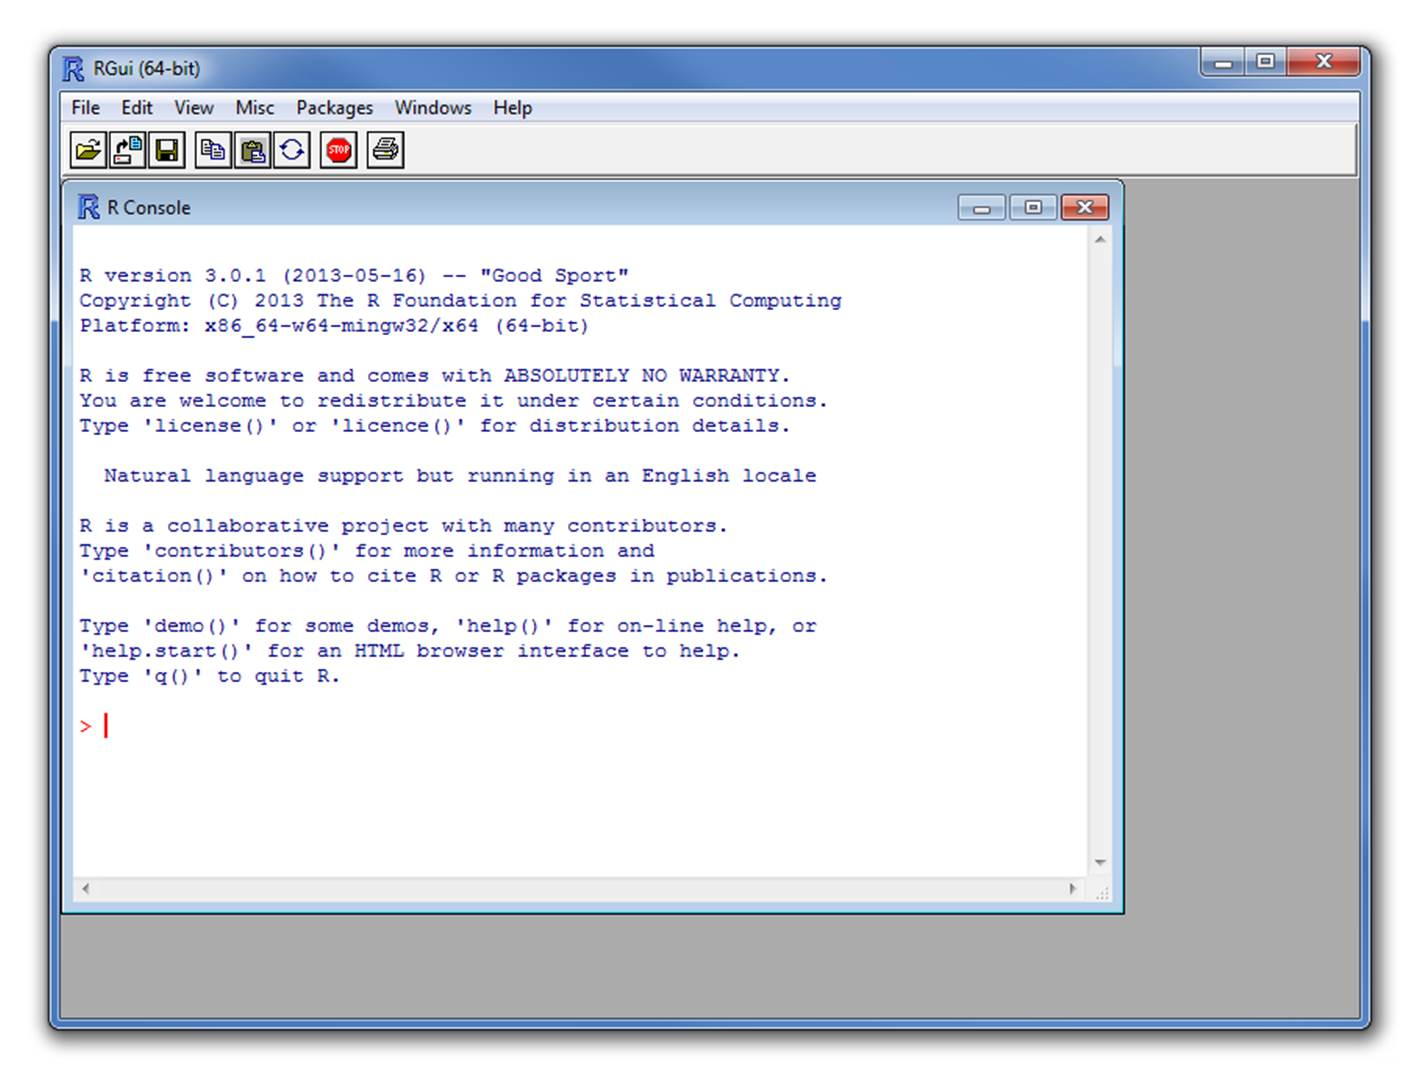
\includegraphics[width=0.5\textwidth]{Bilder/R_Konsole.jpg}
  \item Tipp: Mit der Basis-Software \texttt{R} zu arbeiten ist wenig angenehm. \\ Es empfiehlt sich einen Editor zu benutzen, z.B. RStudio: \href{https://docs.posit.co/ide/user/\#install-links}{\textcolor{MidnightBlue}{https://posit.co/download/rstudio-desktop/}}
\end{enumerate}
\end{frame}

\begin{frame}
\frametitle{Grundlagen -- RStudio}
\begin{center}
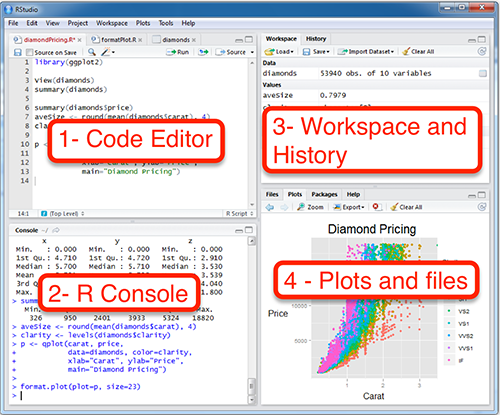
\includegraphics[width=0.65\textwidth]{Bilder/Rstudio}
\end{center}
{\tiny Quelle: http://www.sthda.com/english/wiki/running-rstudio-and-setting-up-your-working-directory-easy-r-programming}
\end{frame}

%-------------- Objektklassen
\section{Objektklassen}
\frame{\frametitle{Objektklassen}\tableofcontents[currentsection, subsectionstyle=show/show/hide]}
\addtocounter{framenumber}{-1}

\begin{frame}[fragile]
\frametitle{Objektklassen}
Jedes Objekt in \texttt{R} hat eine spezifische Klasse. Beispiele:
\begin{lstlisting}
> class(17)
[1] "numeric"
> class("O'zapft is!")
[1] "character"
\end{lstlisting}
\vspace{5px}
In einem \textbf{Vektor} besitzen alle Elemente die selbe Klasse:
\begin{lstlisting}
> a <- c("Ich bin", "ein Vektor mit", 4, "Elementen")
> class(a[3])
[1] "character"
\end{lstlisting}
\vspace{5px}
In einer \textbf{Liste} besitzt jedes Element eine individuelle Klasse:
\begin{lstlisting}
> b <- list("Ich bin", "eine Liste mit", 4, "Elementen")
> class(b[[3]])
[1] "numeric"
\end{lstlisting}
\end{frame}

\begin{frame}[fragile]
\frametitle{Objektklassen -- Type conversion}
Mathematische Operationen können nur auf Objekte mit bestimmten Klassen angewendet werden:
\begin{lstlisting}
> 2 + 2
[1] 4
> 2 + "2"
Error in 2 + "2": non-numeric argument
\end{lstlisting}
\vspace{5px}
Per \textbf{type conversion} kann man die Klasse eines Objektes ändern:
\begin{lstlisting}
> 2 + as.numeric("2")
[1] 4
# Auch moeglich: as.character, as.factor, as.Date, ...
\end{lstlisting}
\end{frame}

\begin{frame}[fragile]
\frametitle{Objektklassen}
Betrachten wir nun Tabellen:
\\
In einer \textbf{Matrix} besitzen alle Elemente die selbe Klasse:
\begin{lstlisting}
> m <- matrix(c("Wort",1,"Wort",9), nrow = 2, byrow = TRUE)
> m
     [,1]   [,2]
[1,] "Wort" "1" 
[2,] "Wort" "9" 
> class(m[,2]) # zweite Spalte
[1] "character"
\end{lstlisting}
\vspace{5px}
In einem \textbf{data frame} besitzt jede Spalte eine individuelle Klasse:
\begin{lstlisting}
> d <- data.frame(Var1 = c("Wort","Wort"), Var2 = c(2,4))
> d
  Var1 Var2
1 Wort    2
2 Wort    4
> class(d[,2]) # zweite Spalte
[1] "numeric"
\end{lstlisting}
\end{frame}


%-------------- Funktionen und Pakete
\section{Funktionen und Pakete}
\frame{\frametitle{Funktionen und Pakete}\tableofcontents[currentsection, subsectionstyle=show/show/hide]}
\addtocounter{framenumber}{-1}

\begin{frame}[fragile]
\frametitle{Benutzung von Funktionen}
Arbeit mit Funktionen
\begin{itemize}
  \item Für bestehende Funktionen: Hilfeseiten benutzen
  \begin{lstlisting}
> ?mean
  \end{lstlisting}
  \item Aufruf einer Funktion:
  \begin{lstlisting}
> sample <- c(2,5,3,17)
> mean(sample)
[1] 6.75
  \end{lstlisting}
  \item Definition einer neuen Funktion:
  \begin{lstlisting}
> do_something <- function(a, b) {
+   result <- a + b
+   return(result)
+ }
> do_something(2,4)
[1] 6
  \end{lstlisting}
\end{itemize}
\end{frame}

\begin{frame}[fragile]
\frametitle{Benutzung von Paketen}
Arbeit mit Paketen
\begin{enumerate}
  \item Finden eines Pakets mit der gewünschten Funktion, z.B. per Google
  \item Installation des Pakets: \textit{nur ein einziges Mal notwendig}
  \begin{lstlisting}
> install.packages("paketXY")
  \end{lstlisting}  
  \item Laden des Pakets: \textit{bei jedem Neustart von \texttt{R} notwendig}
  \begin{lstlisting}
> library("paketXY")  
  \end{lstlisting}
\end{enumerate}
\end{frame}


%-------------- Arbeit mit Daten
\section{Arbeit mit Daten}
\frame{\frametitle{Arbeit mit Daten}\tableofcontents[currentsection, subsectionstyle=show/show/hide]}
\addtocounter{framenumber}{-1}

\begin{frame}[fragile]
\frametitle{Arbeit mit Daten}
Daten einlesen:
\begin{lstlisting}
> dat <- read.table(
+   file   = "Daten/WDI_Daten.csv",
+   header = TRUE,
+   sep    = ",",
+   dec    = ".")
\end{lstlisting}
\bigskip \bigskip
Mit Variablen arbeiten:
\begin{lstlisting}
> mean(dat$Area)
[1] 491912.6
> dat$new_variable <- dat$CO2emission / dat$Area
\end{lstlisting}
\end{frame}

\begin{frame}[fragile]
\frametitle{Arbeit mit Daten}
Daten kennenlernen mit \texttt{str()}:
\begin{lstlisting}
> str(dat)
'data.frame':	315 obs. of  8 variables:
 $ country    : Factor w/ 45 levels "Albania","Andorra",..: 2 2 2 2 2 2 2 1 1 1 ...
 $ region     : Factor w/ 4 levels "Eastern Europe",..: 3 3 3 3 3 3 3 3 3 3 ...
 $ year       : int  2005 2006 2007 2008 2009 2010 2011 2005 2006 2007 ...
 $ CO2emission: num  576 546 539 539 517 ...
 $ Population : int  81223 83373 84878 85616 85474 84419 82326 3011487 2992547 2970017 ...
 $ Area       : int  470 470 470 470 470 470 470 27400 27400 27400 ...
 $ BevDichte  : num  173 177 181 182 182 ...
 $ LandJahr   : Factor w/ 315 levels "Albania_2005",..: 8 9 10 11 12 13 14 1 2 3 ...
\end{lstlisting}
\end{frame}

\begin{frame}[fragile]
\frametitle{Arbeit mit Daten - Visualisierung}
Hier einzelne Beispiele auf Basis des \texttt{ggplot2} Pakets:
\begin{lstlisting}
> library(ggplot2)
> theme_set(theme_bw()) # globales Plot-Theme setzen

> ggplot(dat, aes(x = region)) + 
+   geom_bar()
> ggplot(dat, aes(x = year, y = CO2emission)) +
+   geom_point()
> ggplot(dat, aes(x = year, y = CO2emission, color = country)) +
+   geom_line()
\end{lstlisting}
\bigskip \bigskip
Auf der Suche nach Inspiration? Siehe die \href{http://www.r-graph-gallery.com/}{\textcolor{MidnightBlue}{R Graph Gallery}}.
\end{frame}

\begin{frame}
\frametitle{Arbeit mit Daten - Best Practices}
Workflow für eine Analyse:
\begin{enumerate}
  \item Erstelle eines Projektordners in welchen man Code und Daten legt
  \item Arbeite mit einer \texttt{.R}-Datei und nicht in der Konsole
  \item Erster Schritt: Setze das Arbeitsverzeichnis per \texttt{setwd()} \\ {\tiny Anm.: In Windows muss man die Slashes im Pfad umdrehen!}
  \item Erster Schritt nach dem Einlesen der Daten: \\ Stelle sicher, dass jede Variable die korrekte Klasse hat. \\ Falls nicht der Fall, nutze \texttt{as.numeric()}, \texttt{as.factor()} etc.
  \item Führe die Datenaufbereitung komplett in \texttt{R} durch (automatische Reproduzierbarkeit!) und nicht in Excel
  \item Nutze Kommentare im Code, um zu beschreiben was der Code macht!
\end{enumerate}
\end{frame}



%-------------- Weitere Materialien
\section{Weitere Materialien}
\frame{\frametitle{Weitere Materialien}\tableofcontents[currentsection, subsectionstyle=show/show/hide]}
\addtocounter{framenumber}{-1}

% \begin{frame}[fragile]\frametitle{Summing things up - Useful functions}
% \begin{tabular}{ll}
% \toprule
%   Command & Functionality \\
% \midrule
%   \texttt{<-} / \texttt{=} & Assignment in R \\
%   \texttt{c()} & Put multiple elements in one vector \\
%   \texttt{seq()} & Generate numberic sequences \\
%   \texttt{rep()} & Generate general sequances \\
%   \texttt{length()}  & Length of an object \\
%   \texttt{getwd()}  & Get current path (\textbf{w}orking \textbf{d}irectory) \\
%   \texttt{setwd()}  & Set current path (\textbf{w}orking \textbf{d}irectory) \\
%   \texttt{ls()}  & Shows all objects in the workspace \\
%   \texttt{rm(list=ls())} & Delete all objects from the workspace \\
%   \texttt{?log} & Call help page for function \texttt{log()}\\
%   \texttt{citation()} & Citation info for \texttt{R} itself or specific packages  \\
% \bottomrule
% \end{tabular}
% \end{frame}
% 
% \begin{frame}[fragile]\frametitle{Summing things up - Useful functions II} 
% \begin{tabular}{ll}
% \toprule
%   Command & Functionality \\
% \midrule
%   \texttt{summary()}    & Useful information regarding the object \\
%   \texttt{str()}        & Even more useful information \\
%   \texttt{which()}      & Get indices, at which a vector is \texttt{TRUE} \\
%   \texttt{paste()}      & Paste two character objects together \\
%   \texttt{head()}       & Show only the first elements of an object \\
%   \texttt{dim()}        & Get the dimensions of a dataset\\
%   \texttt{names()}      & Get the names of a dataset\\
%   \texttt{cbind()}      & Merge two datasets regarding the columns\\
%   \texttt{rbind()}      & Merge two datasets regarding the rows\\
%   \texttt{load()}       & Load an object (as \texttt{.RData}) \\
%   \texttt{save()}       & Save an object (as \texttt{.RData}) \\
% \bottomrule
% \end{tabular}
% \end{frame}


\begin{frame}
\frametitle{Weitere Materialien}
Zusätzliche hilfreiche Materialien:
\begin{itemize}
  \item \href{https://github.com/saghirb/Getting-Started-in-R}{\textcolor{MidnightBlue}{Getting started in R}}
  \item \href{https://posit.co/resources/cheatsheets/}{\textcolor{MidnightBlue}{Cheatsheets}} von Posit
\end{itemize}
\bigskip \bigskip \bigskip
\begin{center}
{\Large Weitere Fragen?}
\\[0.5cm]
$\Rightarrow$ fragt die KI eures Vertrauens
\end{center}
\end{frame}

\end{document}